\hypertarget{_font_proportionality_8h}{
\section{FontProportionality.h File Reference}
\label{_font_proportionality_8h}\index{FontProportionality.h(114)@{FontProportionality.h(114)}}
}


\subsection{Detailed Description}
Declaration of enumeration FontProportionality. 



Definition in file \hyperlink{_font_proportionality_8h-source}{FontProportionality.h}.



This graph shows which files directly or indirectly include this file:\nopagebreak
\begin{figure}[H]
\begin{center}
\leavevmode
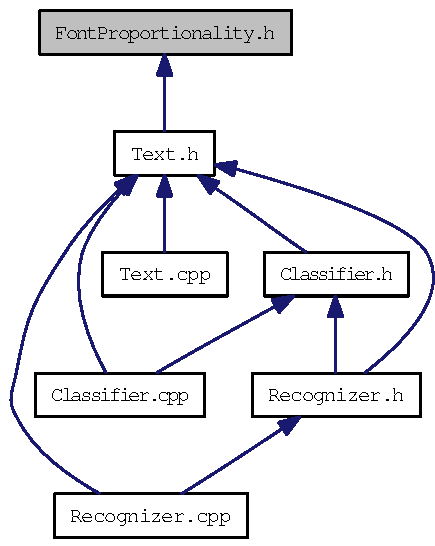
\includegraphics[width=122pt]{_font_proportionality_8h__dep__incl}
\end{center}
\end{figure}
\subsection*{Enumerations}
\begin{CompactItemize}
\item 
enum \hyperlink{_font_proportionality_8h_a9aa255df24db58a9b4cbc46941f2ac1}{FontProportionality} \{ \hyperlink{_font_proportionality_8h_a9aa255df24db58a9b4cbc46941f2ac1dc1e8f9aeb4699a239362b100670de62}{FONT\_\-MONOSPACED}, 
\hyperlink{_font_proportionality_8h_a9aa255df24db58a9b4cbc46941f2ac1923ae135c613560cceef2568bd9cfa8d}{FONT\_\-PROPORTIONAL}
 \}
\begin{CompactList}\small\item\em Font proportionality of a character. \item\end{CompactList}\end{CompactItemize}


\subsection{Enumeration Type Documentation}
\hypertarget{_font_proportionality_8h_a9aa255df24db58a9b4cbc46941f2ac1}{
\index{FontProportionality.h@{FontProportionality.h}!FontProportionality@{FontProportionality}}
\index{FontProportionality@{FontProportionality}!FontProportionality.h@{FontProportionality.h}}
\subsubsection[FontProportionality]{\setlength{\rightskip}{0pt plus 5cm}enum {\bf FontProportionality}}}
\label{_font_proportionality_8h_a9aa255df24db58a9b4cbc46941f2ac1}


Font proportionality of a character. 

This enumeration represents the different types of font proportionality that a text may have. The monospaced type is usual in fixed width fonts, while proportional type is usual in Roman fonts.

\begin{Desc}
\item[Author:]Eliezer Talón (\href{mailto:elitalon@gmail.com}{\tt elitalon@gmail.com}) \end{Desc}
\begin{Desc}
\item[Date:]2008-09-23 \end{Desc}
\begin{Desc}
\item[Enumerator: ]\par
\begin{description}
\index{FONT\_\-MONOSPACED@{FONT\_\-MONOSPACED}!FontProportionality.h@{FontProportionality.h}}\index{FontProportionality.h@{FontProportionality.h}!FONT\_\-MONOSPACED@{FONT\_\-MONOSPACED}}\item[{\em 
\hypertarget{_font_proportionality_8h_a9aa255df24db58a9b4cbc46941f2ac1dc1e8f9aeb4699a239362b100670de62}{
FONT\_\-MONOSPACED}
\label{_font_proportionality_8h_a9aa255df24db58a9b4cbc46941f2ac1dc1e8f9aeb4699a239362b100670de62}
}]In fixed width fonts. \index{FONT\_\-PROPORTIONAL@{FONT\_\-PROPORTIONAL}!FontProportionality.h@{FontProportionality.h}}\index{FontProportionality.h@{FontProportionality.h}!FONT\_\-PROPORTIONAL@{FONT\_\-PROPORTIONAL}}\item[{\em 
\hypertarget{_font_proportionality_8h_a9aa255df24db58a9b4cbc46941f2ac1923ae135c613560cceef2568bd9cfa8d}{
FONT\_\-PROPORTIONAL}
\label{_font_proportionality_8h_a9aa255df24db58a9b4cbc46941f2ac1923ae135c613560cceef2568bd9cfa8d}
}]In Roman fonts. \end{description}
\end{Desc}



Definition at line 20 of file FontProportionality.h.